\section{Reproducible numerical example}
\label{sec:results}
The default experiment uses
\begin{equation}
 \epsilon=10^{-4},\quad\sigma=0.18,\quad\eta_o=1.8,\quad
 \chi_o=0.65,\quad s_0=1.3.
\end{equation}
The unperturbed emission time is $\eta_e=0.5$.
The main nonradial comparison uses $\alpha_0=0.25$ radians.
The entire background interval is expanding; no ray crosses a turnaround.
The largest Newtonian-gauge density contrast at reception is below
$0.4\%$. The sampled maximum peculiar speed is
$\MaxPeculiarSpeed\times10^{-6}c$. Both the matter perturbations and
the potential remain small in this experiment.

\begin{table}[htbp]
 \centering\small
 \begin{tabular}{@{}p{0.65\linewidth}r@{}}
 \toprule
 Quantity & Computed value\\
 \midrule
 Core comoving density contrast & $\CoreDensityPercent\%$\\
 Core lapse $N_o$ & $\CoreLapse$\\
 Positive-core radius $\chi_c$ (rad) & $\CoreRadius$\\
 $GM_+/(c^2A_{\max})$, in units of $10^{-6}$ & $\CoreMassScaled$\\
 Core clock offset, in units of $10^{-6}A_{\max}/c$ & $\CoreClockOffset$\\
 Radial additional lookback $\Delta s$, in units of $10^{-6}$ & $\RadialDelay$\\
 First-order integral for $\Delta s$, in units of $10^{-6}$ & $\BornDelay$\\
 Matched-source angular shift at $\alpha_0=0.25$ ($\mu$rad) & $\AngularShift$\\
 First-order angular integral ($\mu$rad) & $\BornAngularShift$\\
 Fitted power of the timing remainder versus $\epsilon$ & $\RemainderPower$\\
 \bottomrule
 \end{tabular}
 \caption{Illustrative dimensionless results, generated directly from
 the calculation. These are not measurements or predictions for an
 identified astronomical object. The clock interval is $0.4\leq\eta\leq1.8$.}
 \label{tab:results}
\end{table}

The positive-core mass uses Eq.~\eqref{eq:mass}. Since its value depends
on the source evolution and the specified density contrast, it should
not be interpreted as a conserved Schwarzschild mass.
The ray integrator agrees with the independent radial integral through
first order. Varying $\epsilon$ from $2.5\times10^{-5}$ to
$4\times10^{-4}$ gives a remainder proportional to
$\epsilon^{\RemainderPower}$, as expected for the terms retained by
integrating the truncated metric beyond first order.

\begin{figure}[htbp]
 \centering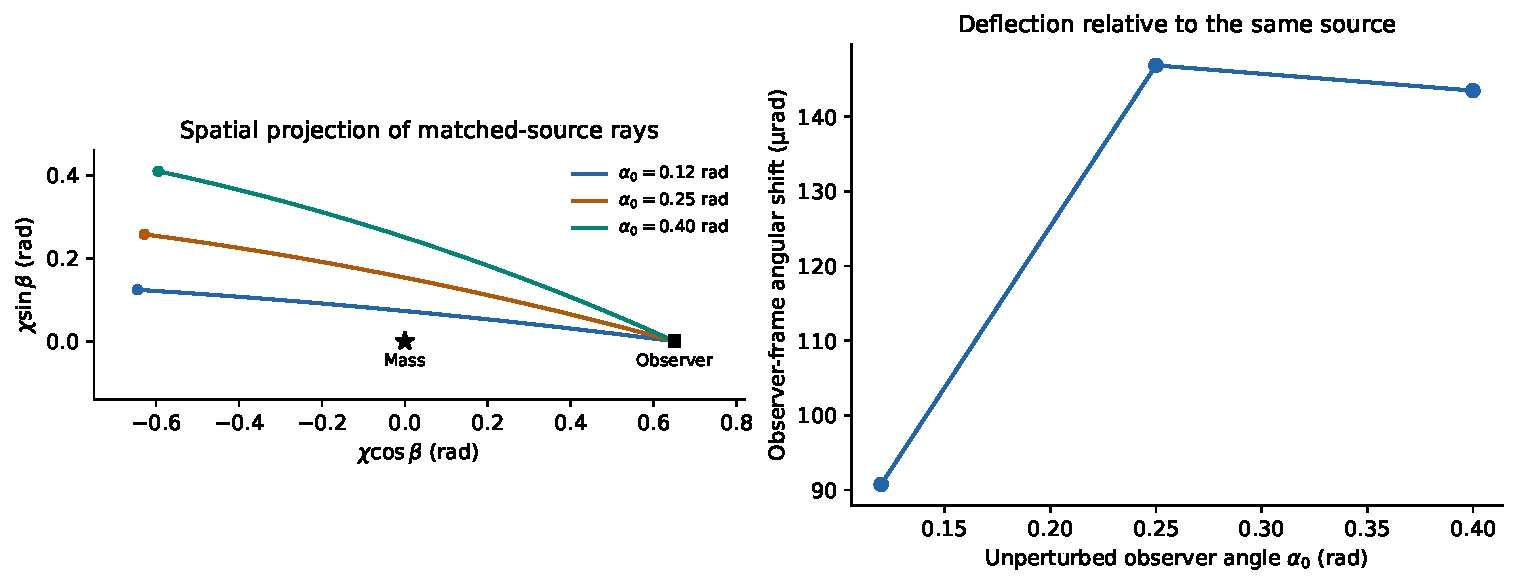
\includegraphics[width=\linewidth]{04-matched-light-rays.pdf}
 \caption{Spatial projections and observer-frame angular shifts for
 three matched sources. The left panel is a normal-coordinate drawing
 on a two-sphere section, with each dot representing its source. Physical
 deflections are too small to distinguish reliably by overplotting paths
 at this scale; the right panel reports the computed angular differences.
 The horizontal axis on the right is the baseline sky angle, not the
 temporal--radial drawing angle.}
 \label{fig:lensing}
\end{figure}
\begin{figure}[htbp]
 \centering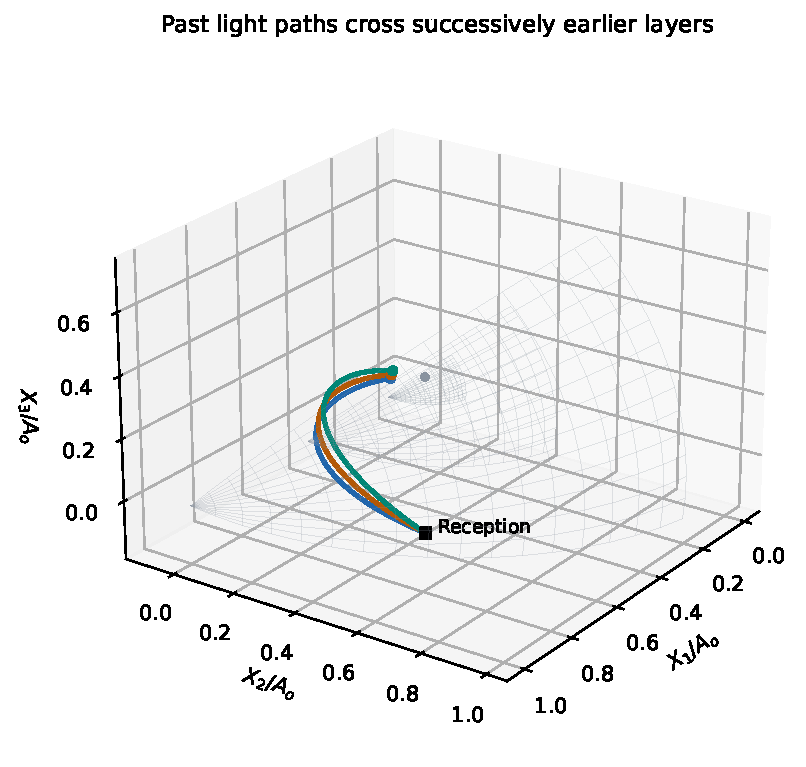
\includegraphics[width=0.78\linewidth]{05-nested-view-lines.pdf}
 \caption{The matched-source view lines in a three-coordinate section
 of the four-dimensional background embedding. Wireframes represent
 portions of the same two-sphere section at $\eta=0.65,1.2,1.8$.
 Each three-dimensional spatial universe is a three-sphere; the mesh
 shown is only a two-dimensional section of it. The radius labels time
 through $A(\eta)$, and spatial deformation is shown separately in
 Fig.~\ref{fig:deformation}. Following a line away from reception takes
 it inward through the history.}
 \label{fig:nested}
\end{figure}
\begin{figure}[htbp]
 \centering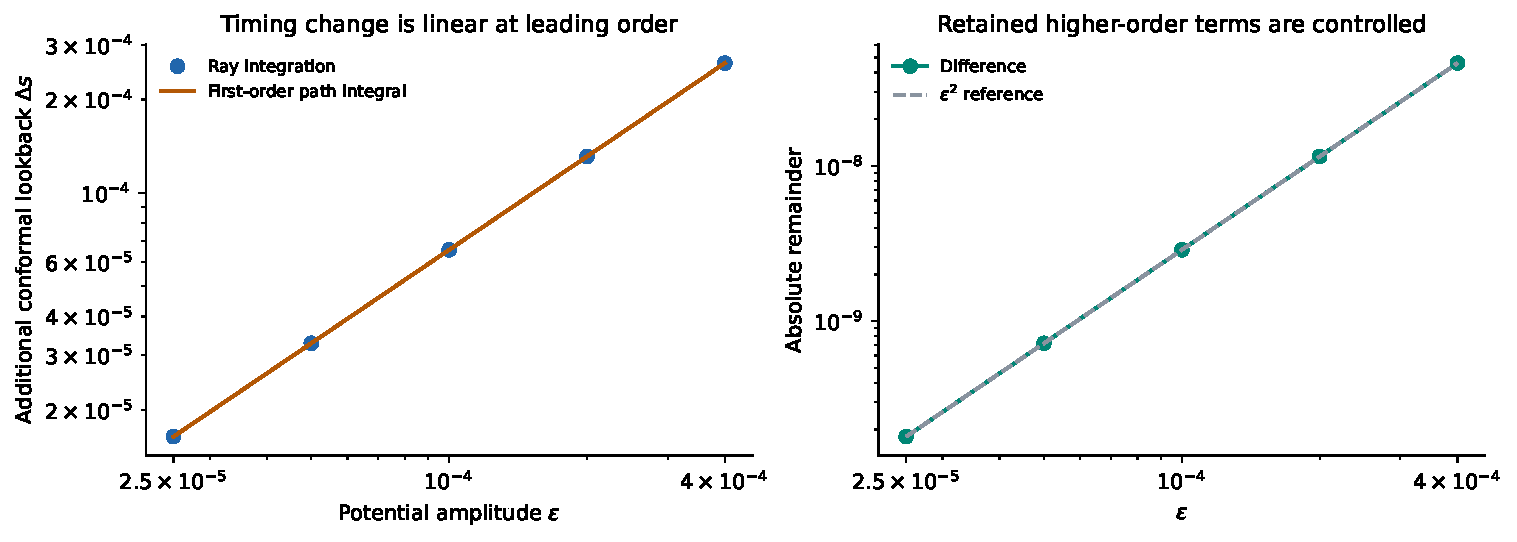
\includegraphics[width=\linewidth]{06-delay-convergence.pdf}
 \caption{Radial timing comparison and amplitude convergence. The
 difference between the integrated truncated-metric result and the
 first-order path integral scales quadratically with potential amplitude.
 This tests perturbative consistency; it does not validate missing
 second-order Einstein dynamics.}
 \label{fig:convergence}
\end{figure}

\subsection{Checks and reproducibility}
The repository contains reusable Python modules, not only figure scripts.
The numerical tests cover the background Friedmann relation, proper-time
normalization, an independent integral for the growth mode, global
compensation, the sphere Laplacian, perturbation sizes, the unperturbed
great-circle and redshift limits, ray constraints, angular-momentum
conservation, timing convergence, reflected source matching, and solver
tolerance stability. Symbolic tests check dust continuity and Euler
evolution, the closed-dust potential coefficient, the induced spatial
metric, and first-order lapse and optical-speed expansions.
Independent angular and frequency integrals also check the deflection
and the endpoint/integrated-potential contributions to redshift.

All figure files, CSV data, diagnostic JSON, and the numerical macros in
Table~\ref{tab:results} are regenerated by \texttt{make results}.
The paper is built by \texttt{make paper}, and the complete check/build
sequence by \texttt{make all}. Version pins are recorded in
\texttt{requirements.lock}; the diagnostic JSON records the scientific
package versions actually used. The default numerical parameters are
centralized in the model and reproduction script.
\FloatBarrier
